% Main manuscript for the Ludic AI publication package.
% Compile with pdflatex + bibtex + pdflatex + pdflatex.
\newif\ifneuripsstyle
\IfFileExists{neurips_2026.sty}{\neuripsstyletrue}{\neuripsstylefalse}

\documentclass[10pt]{article}
\ifneuripsstyle
  \usepackage[preprint]{neurips_2026}
\else
  \usepackage[margin=1in]{geometry}
  \usepackage[numbers,sort&compress]{natbib}
\fi

\usepackage[T1]{fontenc}
\usepackage[utf8]{inputenc}
\usepackage{microtype}
\usepackage{booktabs}
\usepackage{amsmath,amssymb,amsthm,mathtools}
\usepackage{graphicx}
\usepackage{xcolor}
\usepackage{enumitem}
\usepackage{hyperref}
\usepackage{cleveref}
\usepackage{tikz}
\usetikzlibrary{arrows.meta,positioning,fit}
\hypersetup{colorlinks=true, citecolor=blue!60!black, linkcolor=blue!60!black, urlcolor=blue!60!black}

\newtheorem{theorem}{Theorem}
\newtheorem{proposition}{Proposition}
\newtheorem{definition}{Definition}
\newtheorem{remark}{Remark}

\newcommand{\E}{\mathbb{E}}
\newcommand{\I}{\mathbb{I}}
\newcommand{\Aset}{\mathcal{A}}
\newcommand{\Sset}{\mathcal{S}}
\newcommand{\Oset}{\Omega}
\newcommand{\Menu}{\mathcal{M}}
\newcommand{\Env}{\mathcal{E}}
\newcommand{\CC}{\mathrm{CC}}
\newcommand{\RPR}{\mathrm{RPR}}
\newcommand{\LI}{\mathrm{LI}}
\newcommand{\VLI}{\mathrm{VLI}}
\newcommand{\LCB}{\mathrm{LCB}}
\newcommand{\UCB}{\mathrm{UCB}}
\newcommand{\CVaR}{\mathrm{CVaR}}
\newcommand{\ConfoundRate}{\mathrm{ConfoundRate}}
\newcommand{\argmax}{\operatorname*{arg\,max}}
\newcommand{\argmin}{\operatorname*{arg\,min}}
\newcommand{\ludic}{\textsc{Ludic AI}}

\title{Ludic AI: A Judge-Free Benchmark for Identifiable Persona-Conditioned Suboptimization in Stochastic Environments}
\author{Anonymous Authors}
\date{}

\begin{document}
\maketitle

\begin{abstract}
Outcome-only evaluation of language-model agents in stochastic interactive environments is non-identifiable: when an agent incurs a utility loss, the evaluator cannot distinguish arithmetic failure, state-tracking failure, illegal action invention, and valid adherence to a behavioral constraint. We introduce \ludic, a judge-free benchmark that makes these cases separable by construction. At each decision state, a rollout oracle audits every legal root action, estimates local action values, and computes empirical Bernstein lower and upper confidence bounds from bounded rollouts. A persona-conditioned selector is then restricted to behavioral choice over grounded alternatives, and a deterministic validity gate accepts the move only if it is parsable, legal, and constraint-consistent. The framework logs the exact local value gap when exact action values are available, the constraint cost $\CC_t^\psi$, the residual persona regret $\RPR_t^\psi$, and the certified validated ludic index
$$
\VLI_t^{\mathrm{cert}} = A_t\bigl[\LCB_t(\hat a_t^\star) - \UCB_t(a_{\mathrm{LLM},t})\bigr]_+.
$$
Two implementation invariants are enforced in code: $\RPR_t^\psi$ is undefined unless $A_t=1$, and turns with feasible-set collapse are excluded from all $\CC_t^\psi$ aggregates rather than coerced to zero. Audit and selection consume independent RNG streams, preventing rollout consumption from altering selector behavior. The result is a competence-controlled evaluation protocol for measuring alignment under objective pressure: how much expected value an agent verifiably forfeits to remain behaviorally consistent when constraint satisfaction is costly.
\end{abstract}

\section{Introduction}
Outcome-centric agent evaluation is epistemically underdetermined. Success rate, return, and downstream completion do not identify \emph{why} a local move was bad. In a stochastic, partially observed, order-sensitive environment, the same realized utility loss can arise from at least four mechanisms: arithmetic failure, state-tracking failure, illegal action invention, and valid adherence to a behavioral constraint. Existing benchmarks measure the loss and discard the cause \citep{liu2023agentbench,zhou2023webarena,hafner2021benchmarking,kuttler2020nethack}. This is acceptable for pure capability evaluation and inadequate for evaluating constrained, steerable behavior.

The failure mode is not philosophical; it is statistical. Let an agent select a suboptimal move in a stochastic environment. Outcome-only evaluation cannot determine whether the move reflects incapacity or successful constraint adherence. Judge-model pipelines do not fix this. They inherit the same long-horizon arithmetic and grounding weaknesses as the actor itself \citep{gu2024llmjudge}. Reward-model or preference-model supervision does not fix it either: reward proxies remain vulnerable to specification error and incomplete local mathematical evaluation \citep{ouyang2022instructgpt,malik2025rewardbench2}. The missing object is a \emph{competence-controlled} benchmark in which local sacrifice is attributable.

We build that object. The key design principle is decoupling. A rollout oracle computes local competence by auditing legal root actions. A persona-conditioned selector performs only behavioral choice over audited alternatives. A deterministic validity gate decides whether the selected move is parsable, legal, and persona-consistent. The metric layer then records only those gaps that survive this gate. The benchmark therefore does not attempt to infer latent intention or ``personality.'' It measures something narrower and stronger: \emph{validated persona-conditioned suboptimization}.

The scientific payoff is a new decomposition of local failure. When the constrained feasible set is nonempty, total local gap separates into an environment-driven \emph{constraint cost} and a selector-driven \emph{residual persona regret}. The former measures how expensive it is to obey the constraint at all. The latter measures how much additional value the selector leaves on the table even within the feasible constrained set. This turns alignment under objective pressure from rhetoric into a measurable quantity.

The released code implements this factorization as a domain-agnostic Python framework. The environment is abstract, the oracle is rollout-based, personas are deterministic predicates over oracle-computed features, selectors are pluggable, the gate is explicit, and the logging schema is fixed. The benchmark supports both online episode evaluation and matched-state evaluation via an audited state bank. The latter is the critical protocol for statistically clean comparisons because it removes downstream trajectory drift.

Our contributions are fourfold. First, we formalize the non-identifiability of outcome-only evaluation for constrained play. Second, we present a rollout-audited, judge-free benchmark with strict audit-selection RNG separation. Third, we define exact, estimated, and certified local quantities, including $\CC_t^\psi$, gated $\RPR_t^\psi$, and empirical-Bernstein-certified $\VLI_t^{\mathrm{cert}}$. Fourth, we provide a fully runnable reference package that exposes the complete code-to-equation mapping, exports reproducible CSV schemas, and demonstrates the benchmark on a stochastic toy environment with exact local values.

\section{Related Work}
\paragraph{Interactive agent benchmarks.}
AgentBench, WebArena, Crafter, and the NetHack Learning Environment evaluate LLM or RL agents in interactive environments via success, completion, or reward \citep{liu2023agentbench,zhou2023webarena,hafner2021benchmarking,kuttler2020nethack}. These benchmarks are valuable because they are difficult, long-horizon, and grounded. They do not isolate validated constrained sacrifice. A failed move is simply a failed move.

\paragraph{Grounded neuro-symbolic systems.}
Grounded language-control systems such as SayCan combine language priors with external competence signals or affordance estimates \citep{ichter2023saycan}. Our benchmark shares the grounding instinct but changes the scientific objective. The oracle is not introduced to improve control performance per se. It is introduced to identify the cause of local suboptimization.

\paragraph{Reasoning-and-acting baselines.}
Prompting schemes such as ReAct improve action quality by interleaving reasoning and acting \citep{yao2023react}. They remain vulnerable to the central identifiability problem: when a generated action is inferior, the evaluator still cannot attribute the error source without grounded alternatives and explicit validation.

\paragraph{Alignment, evaluation, and constraints.}
RLHF and related preference-learning pipelines optimize behavioral proxies rather than externally grounded local values \citep{ouyang2022instructgpt}. Judge-model pipelines are themselves evaluation models and inherit calibration, consistency, and bias concerns \citep{gu2024llmjudge}. Reward-model benchmarks show that evaluation quality remains a live problem even when supervision is explicit \citep{malik2025rewardbench2}. PersonaGym and related work study persona fidelity or role adoption \citep{samuel2024personagym}; pluralistic alignment work emphasizes the need for trade-off-sensitive evaluation \citep{sorensen2024pluralistic}. Constrained Markov decision processes provide the classical language of optimality under additional costs \citep{altman1999cmdp}. \ludic{} is adjacent to CMDPs but operationally different: the benchmark measures the cost of a declared behavioral constraint and the selector's residual error inside the resulting feasible set.

\section{Problem Formulation}
Let the environment be a partially observed stochastic decision process
$$
\Env = (\Sset, \Aset, T, R, \Oset, O, \gamma).
$$
At turn $t$, the latent state is $s_t \in \Sset$, the observable history is $h_t = (o_1,a_1,\ldots,o_t)$, and the benchmark exposes a grounded decision representation $x_t = \phi(h_t)$. The legal root action set is $\Aset_t = \Aset(x_t)$.

For fixed audit horizon $H$, define the local value of action $a \in \Aset_t$ under continuation rollout policy $\rho_{\mathrm{cont}}$ by
$$
Q_t(a) = \E\!\left[\sum_{k=0}^{H-1} \gamma^k r_{t+k} \mid x_t, a_t = a, \rho_{\mathrm{cont}}\right].
$$
The environment may optionally implement an exact local evaluator for $Q_t(a)$. When it does not, the benchmark remains meaningful in estimated and certified form.

The benchmark's core epistemic claim is that outcome-only evaluation is non-identifiable with respect to valid constrained deviation. The statement is elementary but decisive.

\begin{proposition}[Outcome-only non-identifiability]
Assume there exists a decision state $x_t$ and actions $a,b \in \Aset_t$ with $Q_t(a) > Q_t(b)$. Let $\pi^{\mathrm{val}}$ choose $b$ because $b$ satisfies a behavioral constraint and let $\pi^{\mathrm{err}}$ choose $b$ because of internal error. Any evaluator that conditions only on the executed action and realized future trajectory cannot distinguish $\pi^{\mathrm{val}}$ from $\pi^{\mathrm{err}}$ at turn $t$.
\end{proposition}

\begin{proof}
Both policies induce the same conditional trajectory law $p(\tau_{t:T} \mid x_t, a_t = b)$. Any statistic measurable with respect to $(x_t,b,\tau_{t:T})$ therefore has the same distribution under both policies. The latent cause of choosing $b$ is not identifiable from outcome alone.
\end{proof}

The only way out is to introduce additional observable structure. \ludic{} does so by separating competence computation from behavioral selection and by making constraint validity explicit.

\section{Methodology and System Design}
\subsection{Rollout oracle}
At each decision state, the oracle audits every legal root action with bounded rollouts. For action $a$, it observes returns $G_{t,1}(a),\ldots,G_{t,n_t(a)}(a)$ and computes
$$
\hat Q_t(a) = \frac{1}{n_t(a)}\sum_{i=1}^{n_t(a)} G_{t,i}(a),
\qquad
\hat \sigma_t^2(a) = \frac{1}{n_t(a)-1}\sum_{i=1}^{n_t(a)}\bigl(G_{t,i}(a)-\hat Q_t(a)\bigr)^2.
$$
The empirical oracle action is
$$
\hat a_t^\star \in \argmax_{a \in \Aset_t} \hat Q_t(a).
$$
If exact values are available, the benchmark also logs the exact oracle action
$$
a_t^\star \in \argmax_{a \in \Aset_t} Q_t(a).
$$

The oracle additionally computes action attributes such as variance, downside probability, $\CVaR$, immediate reward mean, and environment-defined features. These attributes are not cosmetic; they parameterize the feasible set induced by a persona. The oracle returns an audited action table and, optionally, a presentation menu $\Menu_t \subseteq \Aset_t$ such as the top-$k$ actions by $\hat Q_t(a)$. In the code, this is the \texttt{RolloutOracle.audit()} object \texttt{OracleDecision}.

\subsection{Persona-conditioned selector}
A persona is a deterministic specification over oracle-computed features. Let $z_t(a) \in \mathbb{R}^m$ denote the feature vector of action $a$. A persona $\psi$ defines the feasible constrained set
$$
F_{\psi,t} = \left\{ a \in \Aset_t : c_{\psi,j}(z_t(a), h_t) \le 0 \ \forall j \right\}.
$$
Typical examples include risk-seeking, downside-protective, immediacy-biased, and build-preserving behavior.

The selector receives $x_t$, the audited oracle output, the persona specification, and history, then emits one action proposal
$$
a_{\mathrm{LLM},t} \sim \pi_\theta(\cdot \mid x_t, \Menu_t, \psi, h_t).
$$
The selector does not estimate values. Its role is purely behavioral: choose one grounded action consistent with the persona. In the codebase this abstraction is realized by \texttt{BaseSelector}, with \texttt{AbstractLLMMenuSelector} as the provider-facing hook and toy selectors for grounded and ungrounded baselines.

\subsection{Deterministic validity gate}
The benchmark's interpretability boundary is the validity gate. Let \texttt{parse}, \texttt{legal}, and \texttt{persona} be indicators that the selector output can be parsed, is legal in the environment, and satisfies the persona predicate. The core gate is
$$
A_t = \I[\mathrm{parse}_t = 1] \cdot \I[\mathrm{legal}_t = 1] \cdot \I[\mathrm{persona}_t = 1].
$$
The implementation also supports a strict menu-membership variant, but the theorem-bearing path only requires parse, legality, and persona consistency.

This gate is the single most important anti-confound device in the system. Without it, positive value gaps caused by unparsable or illegal actions would contaminate the metric and be misread as behavioral sacrifice.

\subsection{RNG separation}
Audit and selection must be stochastically disjoint. At each decision state, the patched implementation samples two child seeds from a master RNG and instantiates two independent generators,
$$
u_t^{\mathrm{audit}}, u_t^{\mathrm{sel}} \sim \mathrm{MasterRNG},
$$
then gives $u_t^{\mathrm{audit}}$ exclusively to the oracle and $u_t^{\mathrm{sel}}$ exclusively to the selector. This prevents the selector's behavior from changing when oracle rollout depth, rollout count, or action ordering changes. The separation is implemented in \texttt{DecisionEvaluator.evaluate\_state()} and \texttt{StateBankBuilder.collect()}.

\section{Metrics and Theorems}
\subsection{Exact and estimated local gaps}
When exact local values are available, the benchmark logs the exact local value gap
$$
\mathrm{TrueGap}_t = Q_t(a_t^\star) - Q_t(a_{\mathrm{LLM},t}).
$$
For raw diagnostic purposes it also logs an estimated gap
$$
\widehat{\mathrm{Gap}}_t = \hat Q_t(\hat a_t^\star) - \hat Q_t(\tilde a_t),
$$
where $\tilde a_t = a_{\mathrm{LLM},t}$ if the selected action is auditable and otherwise $\tilde a_t$ is an invalid-action proxy fixed at the environment's invalid-action reward floor. The raw Ludic Index is then
$$
\LI_t = \bigl[\widehat{\mathrm{Gap}}_t\bigr]_+.
$$
This quantity is intentionally permissive and therefore not theorem-bearing; its purpose is to expose confounded positive gaps.

\subsection{Constraint cost and residual persona regret}
If $F_{\psi,t} \neq \varnothing$, define the constrained oracle action
$$
a_t^{\psi,\star} \in \argmax_{a \in F_{\psi,t}} Q_t(a).
$$
The exact local decomposition is
$$
Q_t(a_t^\star) - Q_t(a_{\mathrm{LLM},t})
=
\underbrace{Q_t(a_t^\star) - Q_t(a_t^{\psi,\star})}_{\CC_t^\psi}
+
\underbrace{Q_t(a_t^{\psi,\star}) - Q_t(a_{\mathrm{LLM},t})}_{\RPR_t^\psi}.
$$
The first term,
$$
\CC_t^\psi := Q_t(a_t^\star) - Q_t(a_t^{\psi,\star}),
$$
is the \emph{constraint cost}. It measures the irreducible environment-driven cost of obeying the persona. The second term,
$$
\RPR_t^\psi := Q_t(a_t^{\psi,\star}) - Q_t(a_{\mathrm{LLM},t}),
$$
is the \emph{residual persona regret}. It measures the avoidable error of the selector within the feasible set.

The code enforces two domain restrictions. First,
$$
A_t = 0 \Longrightarrow \RPR_t^\psi = \mathrm{NaN}.
$$
An illegal or unparsable move is not regret \emph{within} the feasible constrained set. Second, feasible-set collapse remains undefined rather than zero-filled:
$$
F_{\psi,t} = \varnothing \Longrightarrow \CC_t^\psi = \RPR_t^\psi = P_t^\psi = \mathrm{NaN}.
$$
This prevents strict personas from being misreported as cost-free.

\subsection{Empirical Bernstein confidence intervals}
Let audited returns for action $a$ lie in $[L_t,U_t]$ with width $B_t = U_t - L_t$. The patched oracle uses an empirical Bernstein radius
$$
\beta_t(a,\delta)
=
\hat \sigma_t(a)\sqrt{\frac{2\log(3|\Aset_t|/\delta)}{n_t(a)}}
+
\frac{3B_t\log(3|\Aset_t|/\delta)}{n_t(a)}.
$$
The interval is
$$
\LCB_t(a) = \hat Q_t(a) - \beta_t(a,\delta),
\qquad
\UCB_t(a) = \hat Q_t(a) + \beta_t(a,\delta),
$$
clipped to $[L_t,U_t]$. Compared with Hoeffding-style bounds, this interval adapts to empirical variance and therefore materially tightens certification when local rollout variance is small.

\subsection{Certified validated sacrifice}
The theorem-bearing metric is the certified Validated Ludic Index,
$$
\VLI_t^{\mathrm{cert}} = A_t\bigl[\LCB_t(\hat a_t^\star) - \UCB_t(a_{\mathrm{LLM},t})\bigr]_+.
$$
The operational but less conservative variant is
$$
\VLI_t^{\mathrm{op}} = A_t\bigl[\LCB_t(\hat a_t^\star) - \hat Q_t(a_{\mathrm{LLM},t})\bigr]_+.
$$

\begin{theorem}[High-probability soundness]
Assume each audited root action has independent bounded rollouts and that the empirical Bernstein intervals satisfy simultaneous coverage over all audited root actions with probability at least $1-\delta$. Then on the coverage event,
$$
0 \le \VLI_t^{\mathrm{cert}} \le A_t\bigl[Q_t(\hat a_t^\star) - Q_t(a_{\mathrm{LLM},t})\bigr]_+.
$$
\end{theorem}

\begin{proof}
On the simultaneous coverage event,
$$
\LCB_t(\hat a_t^\star) \le Q_t(\hat a_t^\star),
\qquad
Q_t(a_{\mathrm{LLM},t}) \le \UCB_t(a_{\mathrm{LLM},t}).
$$
Therefore
$$
\LCB_t(\hat a_t^\star) - \UCB_t(a_{\mathrm{LLM},t})
\le
Q_t(\hat a_t^\star) - Q_t(a_{\mathrm{LLM},t}).
$$
Applying the positive-part operator preserves the inequality, and multiplying by $A_t \in \{0,1\}$ preserves nonnegativity and validity filtering.
\end{proof}

The theorem formalizes the benchmark's conservative semantics: certification is impossible unless the selected action is valid \emph{and} the oracle-best action dominates it after accounting for audit uncertainty.

\section{Experimental Setup}
\subsection{Codebase and execution modes}
The released package is domain-agnostic. \texttt{POMDPEnv} defines the minimal environment interface, \texttt{RolloutOracle} audits local actions, \texttt{Persona} constructs deterministic feasible sets, \texttt{BaseSelector} abstracts behavioral policies, \texttt{DeterministicValidityGate} enforces interpretability, \texttt{MetricEngine} computes local quantities, and \texttt{TurnLog} plus \texttt{ExperimentAnalyzer} export the full statistical surface. The framework supports two execution modes.

In \emph{online episode mode}, the selector's chosen action is executed and the environment evolves. This mode measures ecological behavior, invalid-action collapse, and end-to-end return. In \emph{matched-state mode}, the system first constructs an audited state bank
$$
D_{\mathrm{bank}} = \{(x_t,\Aset_t,\mathcal{O}_t,h_t)\}_{t=1}^N,
$$
then re-evaluates multiple selectors and personas on frozen state snapshots with \texttt{execute\_action=False}. This mode removes trajectory drift and is the correct protocol for testing $\CC_t^\psi$ versus pressure and $\RPR_t^\psi$ versus capability.

\subsection{Reference environment}
The package ships with a small stochastic toy environment containing four legal actions: \texttt{safe}, \texttt{risky}, \texttt{setup}, and \texttt{cash\_out}. The environment is intentionally simple and mathematically auditable. It has a latent favorable/unfavorable state, a noisy signal, build-up dynamics through repeated \texttt{setup} actions, and a delayed realization trade-off through \texttt{cash\_out}. The environment implements exact local values, making it suitable for sanity-checking the benchmark's exact and certified metrics.

This reference environment is not the benchmark's conceptual limit; it is the smallest environment that exhibits the required phenomena: local stochastic trade-offs, a nontrivial feasible set under personas, and observable divergence between unconstrained and constrained play.

\subsection{Selectors, personas, and hypotheses}
The package ships with both grounded and ungrounded baselines. The ungrounded baseline is a free-form random selector that may emit invalid or illegal actions. The grounded baselines are capability-scaled selectors that consume the audited menu and stochastically interpolate between poor and good constrained choices. The persona family includes neutral, risk-seeking, loss-averse, and build-preserving conditions, each parameterized by a pressure value.

The primary hypotheses are:
$$
\frac{\partial}{\partial \lambda} \E[\CC_t^\psi(\lambda)] > 0
$$
for increasing persona pressure $\lambda$, and
$$
\frac{\partial}{\partial c} \E[\RPR_t^\psi \mid A_t = 1] < 0
$$
for increasing selector capability $c$.

The epistemic-disentanglement diagnostic is
$$
\ConfoundRate = \frac{\sum_t \I[\LI_t > 0 \land A_t = 0]}{\sum_t \I[\LI_t > 0]}.
$$
This measures how many positive raw gaps are actually uninterpretable invalid deviations.

\section{Results}
We report results from the shipped reference environment and its matched-state bank. These experiments are intended as a benchmark sanity check rather than the final large-scale empirical story. Their role is to verify that the patched implementation behaves in the direction predicted by the theory.

\subsection{Grounding removes confounded positive gaps}
The first result is decisive. In online episode evaluation, the ungrounded free-form baseline exhibits confound rates between $0.67$ and $1.00$ across persona settings, with invalid-action rate $0.53$. Every grounded selector drives both invalid-action rate and confound rate to $0.00$ in the reference runs. This is exactly the benchmark's intended first-stage behavior: before discussing persona-conditioned sacrifice, the system must eliminate invalid positive gaps.

\begin{figure}[t]
  \centering
  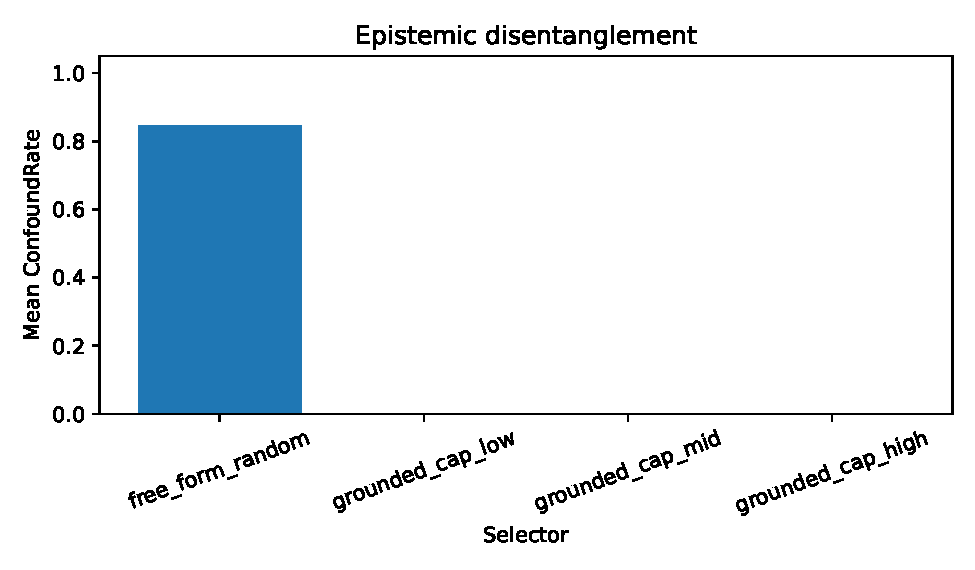
\includegraphics[width=0.78\linewidth]{figures/confound_collapse.pdf}
  \caption{Epistemic disentanglement on the reference environment. Ungrounded play produces large positive raw gaps that are frequently invalid; grounded selectors collapse the confound rate to zero.}
  \label{fig:confound}
\end{figure}

\subsection{Constraint cost rises with persona pressure}
Matched-state evaluation exhibits the expected monotonicity in constraint cost. For the risk-seeking persona, increasing pressure from $0.60$ to $0.85$ raises mean cumulative exact constraint cost from $11.07$ to $16.25$ across grounded selectors. For the loss-averse persona, the same pressure increase raises mean cumulative exact constraint cost from $0.00$ to $0.74$. The trend table exported by the analyzer reports positive OLS slopes for every grounded selector-persona pair in the reference environment.

\begin{figure}[t]
  \centering
  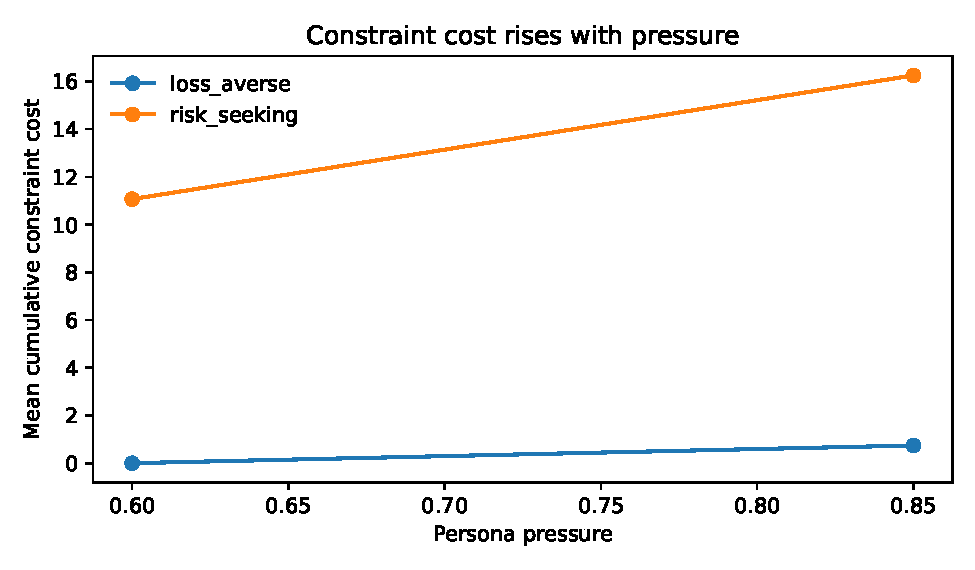
\includegraphics[width=0.78\linewidth]{figures/cc_vs_pressure.pdf}
  \caption{Constraint cost versus persona pressure on the matched-state bank. Pressure increases the cost of behaving according to the declared persona.}
  \label{fig:ccpressure}
\end{figure}

\subsection{Gated residual persona regret falls with capability}
At fixed persona, increasing selector capability reduces gated residual persona regret. In the reference environment, mean cumulative exact $\RPR$ falls from $6.48$ to $0.48$ for build-preserving play, from $7.47$ to $0.48$ for the neutral condition, and from $2.00$ to $0.27$ for risk-seeking play at pressure $0.60$ as capability increases from $0.3$ to $0.9$. The capability trend table reports negative slopes for all informative persona settings in the reference environment.

\begin{figure}[t]
  \centering
  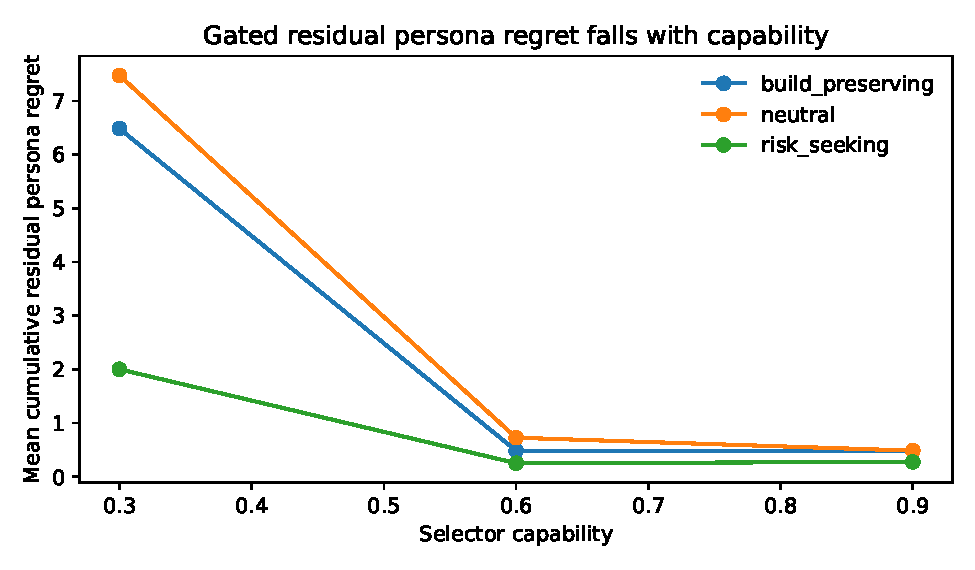
\includegraphics[width=0.78\linewidth]{figures/rpr_vs_capability.pdf}
  \caption{Residual persona regret versus selector capability on the matched-state bank. Higher capability improves action quality within the feasible constrained set.}
  \label{fig:rprcap}
\end{figure}

\subsection{Certification remains conservative in the reference setting}
The reference environment also reveals an important limitation. Although exact local gaps, $\CC$, and gated $\RPR$ behave as intended, the empirical-Bernstein-certified $\VLI_t^{\mathrm{cert}}$ remains zero throughout the shipped sample runs. This is not a logical failure of the metric. It is a power limitation induced by bounded-return width and audit budget. In small environments with wide reward bounds relative to the number of rollouts, certification can remain too conservative to activate. This observation is valuable because it shows that the patched implementation is not generating false positive certified sacrifice; it is, if anything, conservative.

\begin{table}[t]
\centering
\small
\begin{tabular}{p{0.31\linewidth}p{0.58\linewidth}}
\toprule
Diagnostic & Reference result \\
\midrule
Ungrounded confound rate & $0.67$--$1.00$ across personas \\
Grounded confound rate & $0.00$ for all shipped grounded selectors \\
Risk-seeking mean $\sum \CC_t$ & $11.07 \rightarrow 16.25$ as pressure $0.60 \rightarrow 0.85$ \\
Loss-averse mean $\sum \CC_t$ & $0.00 \rightarrow 0.74$ as pressure $0.60 \rightarrow 0.85$ \\
Build-preserving mean $\sum \RPR_t$ & $6.48 \rightarrow 0.48$ as capability $0.3 \rightarrow 0.9$ \\
Neutral mean $\sum \RPR_t$ & $7.47 \rightarrow 0.48$ as capability $0.3 \rightarrow 0.9$ \\
Certified $\sum \VLI_t^{\mathrm{cert}}$ & $0$ in the shipped reference runs \\
\bottomrule
\end{tabular}
\caption{Reference implementation summary from the patched CSV exports. These numbers validate the benchmark mechanics and expose the current certification conservatism in the toy environment.}
\label{tab:summary}
\end{table}

\section{Discussion}
The benchmark's central advance is not that it makes LLM agents stronger. It makes their deviations interpretable. This distinction is easy to blur and essential to preserve. A grounded selector can still be bad; what changes is that a positive gap is no longer silently contaminated by illegal or unparsable moves. Likewise, a persona may genuinely be expensive; the benchmark measures that cost rather than confusing it with model weakness.

The reference implementation also clarifies where the benchmark is strong and where it remains conservative. The exact-gap and exact-decomposition paths are already informative in environments with exact local values. The certified metric is substantially safer than a raw gap, but it may require tighter bounded-return ranges, larger rollout budgets, or better-calibrated environment-specific bounds before it becomes numerically active in small environments. This is a calibration issue, not a conceptual flaw.

The framework inherits several limitations. It is local to audit horizon $H$ and continuation policy $\rho_{\mathrm{cont}}$. Its theorem-bearing path requires personas expressible as deterministic predicates over simulator-computable features. It does not infer latent intention, and it should not be described as doing so. Its strongest form depends on environments that either expose exact local values or yield meaningful audit bounds at practical rollout budgets.

These limitations are acceptable because the benchmark's target is sharply scoped. \ludic{} is not a universal account of agentic alignment. It is a competence-controlled assay for validated suboptimization under objective pressure.

\section{Conclusion}
Outcome-only evaluation collapses invalid moves, capability failures, and valid constrained deviations into the same observable penalty. \ludic{} repairs that collapse by combining a rollout-audited oracle, a persona-conditioned selector, a deterministic validity gate, and a metric layer that distinguishes exact, estimated, and certified local sacrifice. The patched implementation makes the resulting quantities mathematically cleaner: empirical Bernstein intervals replace variance-blind Hoeffding bounds, residual persona regret is undefined outside the valid feasible set, feasible-set collapse is preserved through aggregation, and audit randomness is isolated from selector randomness.

The result is a benchmark for asking a question that standard agent evaluation does not answer: when objective maximization and behavioral consistency diverge, how much verified local value does an agent forgo, and is that loss driven by the environment, by the selector, or by invalid behavior? That is the right unit of analysis for measuring alignment under objective pressure.

\section*{Reproducibility Statement}
The repository accompanying this manuscript contains the complete benchmark code, a fully auditable reference environment, exact CSV schemas for turn-level and episode-level logging, plotting scripts that reproduce the paper figures from exported CSV files, a smoke test, and a super-simple execution guide. All reference-environment results reported in this draft were generated from those exported CSVs.

\begin{thebibliography}{10}

\bibitem[Altman(1999)]{altman1999cmdp}
Eitan Altman.
\newblock \emph{Constrained Markov Decision Processes}.
\newblock Chapman and Hall/CRC, 1999.

\bibitem[Liu et~al.(2023)Liu, Yu, Zhang, Xu, Lei, Lai, Gu, Ding, Men, Yang, et~al.]{liu2023agentbench}
Xiao Liu, Hao Yu, Hanchen Zhang, Yifan Xu, Xuanyu Lei, Hanyu Lai, Yu Gu, Hangliang Ding, Kaiwen Men, Kejuan Yang, et~al.
\newblock AgentBench: Evaluating LLMs as Agents.
\newblock \emph{arXiv preprint arXiv:2308.03688}, 2023.

\bibitem[Zhou et~al.(2023)Zhou, Xu, Zhu, Zhou, Lo, Sridhar, Cheng, Ou, Bisk, Fried, et~al.]{zhou2023webarena}
Shuyan Zhou, Frank F. Xu, Hao Zhu, Xuhui Zhou, Robert Lo, Abishek Sridhar, Xianyi Cheng, Tianyue Ou, Yonatan Bisk, Daniel Fried, et~al.
\newblock WebArena: A Realistic Web Environment for Building Autonomous Agents.
\newblock \emph{arXiv preprint arXiv:2307.13854}, 2023.

\bibitem[Hafner(2021)]{hafner2021benchmarking}
Danijar Hafner.
\newblock Benchmarking the Spectrum of Agent Capabilities.
\newblock \emph{arXiv preprint arXiv:2109.06780}, 2021.

\bibitem[K{"u}ttler et~al.(2020)K{"u}ttler, Nardelli, Miller, Raileanu, McGovern, Tassa, and Grefenstette]{kuttler2020nethack}
Heinrich K{"u}ttler, Nantas Nardelli, Alexander H. Miller, Roberta Raileanu, Brendan McGovern, Thammongkol Tassa, and Edward Grefenstette.
\newblock The NetHack Learning Environment.
\newblock In \emph{Advances in Neural Information Processing Systems}, 2020.

\bibitem[Ichter et~al.(2023)Ichter, Brohan, Chebotar, Finn, Hausman, Herzog, Ho, Ibarz, Irpan, Jang, et~al.]{ichter2023saycan}
Brian Ichter, Anthony Brohan, Yevgen Chebotar, Chelsea Finn, Karol Hausman, Alexander Herzog, Daniel Ho, Julian Ibarz, Alex Irpan, Eric Jang, et~al.
\newblock Do As I Can, Not As I Say: Grounding Language in Robotic Affordances.
\newblock In \emph{Proceedings of The 6th Conference on Robot Learning}, 2023.

\bibitem[Yao et~al.(2023)Yao, Zhao, Yu, Du, Shafran, Narasimhan, and Cao]{yao2023react}
Shunyu Yao, Jeffrey Zhao, Dian Yu, Nan Du, Izhak Shafran, Karthik Narasimhan, and Yuan Cao.
\newblock ReAct: Synergizing Reasoning and Acting in Language Models.
\newblock \emph{arXiv preprint arXiv:2210.03629}, 2023.

\bibitem[Ouyang et~al.(2022)Ouyang, Wu, Jiang, Almeida, Wainwright, Mishkin, Zhang, Agarwal, Slama, Ray, et~al.]{ouyang2022instructgpt}
Long Ouyang, Jeffrey Wu, Xu Jiang, Diogo Almeida, Carroll L. Wainwright, Pamela Mishkin, Chong Zhang, Sandhini Agarwal, Katarina Slama, Alex Ray, et~al.
\newblock Training Language Models to Follow Instructions with Human Feedback.
\newblock \emph{arXiv preprint arXiv:2203.02155}, 2022.

\bibitem[Gu et~al.(2024)Gu, Jiang, Shi, Tan, Zhai, Xu, Li, Shen, Ma, Liu, et~al.]{gu2024llmjudge}
Jiawei Gu, Xuhui Jiang, Zhichao Shi, Hexiang Tan, Xuehao Zhai, Chengjin Xu, Wei Li, Yinghan Shen, Shengjie Ma, Honghao Liu, et~al.
\newblock A Survey on LLM-as-a-Judge.
\newblock \emph{arXiv preprint arXiv:2411.15594}, 2024.

\bibitem[Malik et~al.(2025)Malik, Pyatkin, Land, Morrison, Smith, Hajishirzi, and Lambert]{malik2025rewardbench2}
Saumya Malik, Valentina Pyatkin, Sander Land, Jacob Morrison, Noah A. Smith, Hannaneh Hajishirzi, and Nathan Lambert.
\newblock RewardBench 2: Advancing Reward Model Evaluation.
\newblock \emph{arXiv preprint arXiv:2506.01937}, 2025.

\bibitem[Samuel et~al.(2024)Samuel, Zou, Zhou, Chaudhari, Kalyan, Rajpurohit, Deshpande, Narasimhan, and Murahari]{samuel2024personagym}
Vinay Samuel, Henry Peng Zou, Yue Zhou, Shreyas Chaudhari, Ashwin Kalyan, Tanmay Rajpurohit, Ameet Deshpande, Karthik Narasimhan, and Vishvak Murahari.
\newblock PersonaGym: Evaluating Persona Agents and LLMs.
\newblock \emph{arXiv preprint arXiv:2407.18416}, 2024.

\bibitem[Sorensen et~al.(2024)Sorensen, Moore, Fisher, Gordon, Mireshghallah, Rytting, Ye, Jiang, Lu, Dziri, et~al.]{sorensen2024pluralistic}
Taylor Sorensen, Jared Moore, Jillian Fisher, Mitchell L. Gordon, Niloofar Mireshghallah, Christopher Michael Rytting, Andre Ye, Liwei Jiang, Ximing Lu, Nouha Dziri, et~al.
\newblock Position: A Roadmap to Pluralistic Alignment.
\newblock In \emph{Proceedings of the 41st International Conference on Machine Learning}, 2024.

\end{thebibliography}


\end{document}
